%%%%%%%%%%%%%%%%%%%%%%%%%%%%%%%%%%%%%%%%%%%%%%%%%%%%%%%%%%%%%%%%%%%%%%%%%%%%%%%%
%2345678901234567890123456789012345678901234567890123456789012345678901234567890
%        1         2         3         4         5         6         7         8

\documentclass[letterpaper, 10 pt, conference]{ieeeconf}  % Comment this line out if you need a4paper

%\documentclass[a4paper, 10pt, conference]{ieeeconf}      % Use this line for a4 paper

\IEEEoverridecommandlockouts      


\usepackage{float}                       % This command is only needed if 
\usepackage{graphicx}                                                         % you want to use the \thanks command
\usepackage{subcaption}
\overrideIEEEmargins                                      % Needed to meet printer requirements.

%In case you encounter the following error:
%Error 1010 The PDF file may be corrupt (unable to open PDF file) OR
%Error 1000 An error occurred while parsing a contents stream. Unable to analyze the PDF file.
%This is a known problem with pdfLaTeX conversion filter. The file cannot be opened with acrobat reader
%Please use one of the alternatives below to circumvent this error by uncommenting one or the other
%\pdfobjcompresslevel=0
%\pdfminorversion=4

% See the \addtolength command later in the file to balance the column lengths
% on the last page of the document

% The following packages can be found on http:\\www.ctan.org
%\usepackage{graphics} % for pdf, bitmapped graphics files
%\usepackage{epsfig} % for postscript graphics files
%\usepackage{mathptmx} % assumes new font selection scheme installed
%\usepackage{times} % assumes new font selection scheme installed
%\usepackage{amsmath} % assumes amsmath package installed
%\usepackage{amssymb}  % assumes amsmath package installed

\title{\LARGE \bf
Generación automática de un sketch a lápiz a partir de una fotografía
}


\author{Gibrán Zazueta Cruz}


\begin{document}


\maketitle
\thispagestyle{empty}
\pagestyle{empty}


%%%%%%%%%%%%%%%%%%%%%%%%%%%%%%%%%%%%%%%%%%%%%%%%%%%%%%%%%%%%%%%%%%%%%%%%%%%%%%%%
\begin{abstract}
Se presenta un método que convierte automáticamente cualquier imagen 2D a una imagen con apariencia de un sketch realizado a lápiz. Para ello se utilizan utilizan técnicas de extracción de regiones de interés, para simular el proceso de abstracción de información de una escena que realiza un dibujante, y técnicas de renderizado no-fotorrealista, basadas en generación de trazos mediante extracción de bordes y generación de sombras mediante extracción de tonos.

Los resultados experimentales muestran que las imágenes producidas llegan a ser valoradas como imágenes de buena estética y capaces de simular la apariencia de un sketch a lápiz.
\end{abstract}


%%%%%%%%%%%%%%%%%%%%%%%%%%%%%%%%%%%%%%%%%%%%%%%%%%%%%%%%%%%%%%%%%%%%%%%%%%%%%%%%
\section{INTRODUCCIÓN}

Un dibujo puede llegar a tener la capacidad de mostrar información de una manera más efectiva que una fotografía o incluso un texto escrito.

Parte importante del trabajo del artista es saber extraer información clara de su ambiente y ser capaz de abstraerla y representarla con claridad y estilo. La capacidad que tiene el humano de hacer esto es algo que una computadora aún no es capaz de hacer del todo. Este tipo de problema entra dentro de los  trabajos que son más fáciles para un humano que para una computadora.

En este trabajo se presenta una técnica para hacer una conversión automática de una fotografía a una imagen que imite las características de un sketch a lápiz. Para su resolución se emplean técnicas de renderizado no fotorrealista (NPR), área de la compuación gráfica que desde los 90's ha visto gran crecimiento.

Existen muchos trabajos enfocados en NPR que proponen soluciones para el renderizado de lápiz. Destacados son los artículos de Mao et al.\cite{mao}, que presentó una técnica de renderizado basada en LIC (Linear Integral Convolution), y Lu et al.\cite{lu} que propuso un modelo que genera lineas y sombreado por separado. Ambos reabajos han tenido gran influencia en el área.

Por otro lado, la solución propuesta también tiene un enfoque de visión y abstracción de información. Por medio de información de saliency se busca emular el trabajo del artista de llevar al receptor de la imagen a concentrarse en el área más relevante de esta. En esta área es de destacar el trabajo de DeCarlo y Santella\cite{dec} que estudiaron y midieron la manera en que las personas observan fotografías e ilustracions no fotorrealistas. 

Inspirado en ello Hata et al.\cite{hata} propuso un modelo que buscaba rescatar la información relevante de la imagen por medio de un mapa de saliency, para posteriormente generar un renderizado por medio de LIC.

En particular, este trabajo está fuertemente basado en las publicaciones de Hata et al.\cite{hata}, de quienes se retoma su modelo con mapa saliency, y de Lu et al.\cite{lu}, en la parte de generación de un renderizado con apariencia de lápiz por medio de mapas de trazos y tonos.

Sus propuestas se siguen a través del artículo.

\section{MÉTODO}


\subsection{Modelos de atención visual. Extracción de área de interés}
Una característica fundamental en la definición de un dibujo es que presente una abstracción de la información. Es todo un arte crear imágenes con un buen diseño y estructura que te transmitan un mensaje claro y preciso sin causar un esfuerzo cognitivo mayor.
Es por esto que, enfocarse  en una región de interés no solo es un componente estético deseable al crear una imagen con apariencia de dibujo, sino que es un elemento principal al referirse a la forma en que el dibujo, la pintura y otras artes visuales expresan información. 

Con esta justificación es que el método propuesto busca tomar información de la región de interés para  generar sus resultados.

\subsubsection{Saliency Map}
Basado en la idea de extraer la información de interés se presenta un modelo con mapa de saliency.
El modelo utilizado es el de Hou et al.\cite{hou}. Este modelo se basa en ideas de Teoría de la información y  define que la información de una imagen se puede dividir en 'conocimiento previo' e 'innovación'. La primera corresponde a los valores estadísticos que no varían a lo largo de toda la imagen, información redundante. Si removemos esta parte nos quedamos con la informacion que produce mayor interés visual.

Para llevar a cabo esto, el método analiza la representación logaritmo espectral de la  imagen y resuelve la ecuación

 $$R(f) = L(f) -A(f)$$

Donde L(f) es la representación log espectral de una imagen de entrada, A(f) es un modelo fe forma general del logaritmo espectral, calculado por el método y R(f) son las singularidades estadísticas de la imagen, llamadas en el trabajo 'Residuo espectral'. Si tomamos la transformada de Fourier de este residuo se obtiene una imagen llamada Mapa de saliency que contiene la información no trivial de la escena (porción 'inesperada'de una imagen).

En la figura \ref{saliency} se muestra el resultado de esta técnica.

%%%%%%%%%%IMAGEN SALIENCY
\begin{figure}[H]
\centering
    \begin{subfigure}{0.45\linewidth}
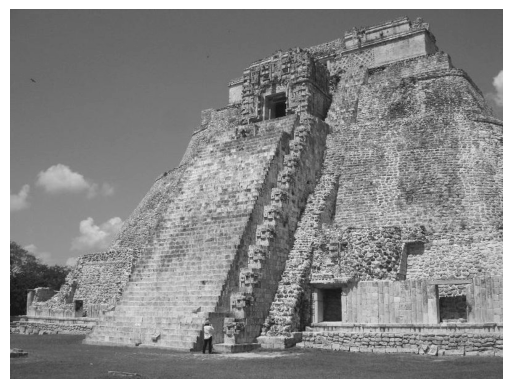
\includegraphics[width=\linewidth, scale=0.05]{images/gray.png}
    \caption{Imagen de entrada en escala de grises}
\label{fig:1a}
    \end{subfigure}\hfill
    \begin{subfigure}{0.45\linewidth}
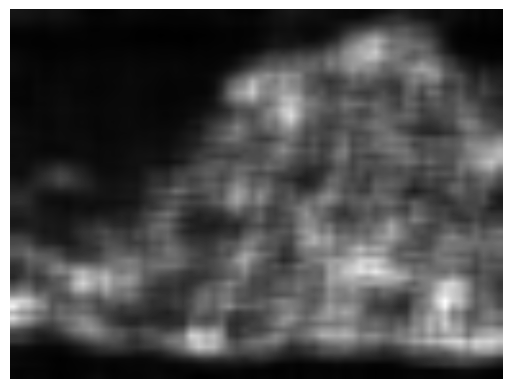
\includegraphics[width=\linewidth, scale=0.05]{images/saliency1.png} 
    \caption{Saliency obtenido por Residuo espectral}
\label{fig:1a}
    \end{subfigure}\hfill
    \begin{subfigure}{0.45\linewidth}
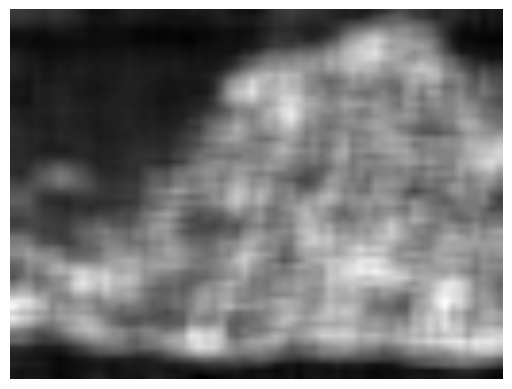
\includegraphics[width=\linewidth, scale=0.05]{images/saliency2.png}
    \caption{Saliency 'expandido'}
\label{saliency}
    \end{subfigure}
\caption{Mapa saliency}
    \label{fig:1}
    \end{figure}
%%%%%%%%%%%%%%%%%%%%%%%%%%%%%%%%


Después de obtener el residuo espectral se saca la raiz cuadrada del mapa obtenido y se le aplica un filtro gaussiano buscando expandir la zona del algoritmo. Esto es debido a que en un dibujo no solo se dibuja el objeto principal de la escena sino que es importante darle contexto a la imagen con la información de su alrededor. En la figura \ref{saliency} se muestra el mapa Saliency 'expandido'



\subsubsection{Multi-resolution image}
Se busca utilizar esta información de saliency, destacando mayor detalle en las partes importantes de la imagen e ir disminuyendo gradualmente. En la figura \ref{ej_sal} se puede ver un ejemplo de un dibujo real con el efecto que se quiere lograr. Como se puede observar, la idea es tener un claro contraste en las áreas de gran interés y gradualmente ir disminuyendo el contraste de la imagen hacia áreas de poco interés.


%%%%%%%%%%IMAGEN SALIENCY
\begin{figure}[H]
\centering
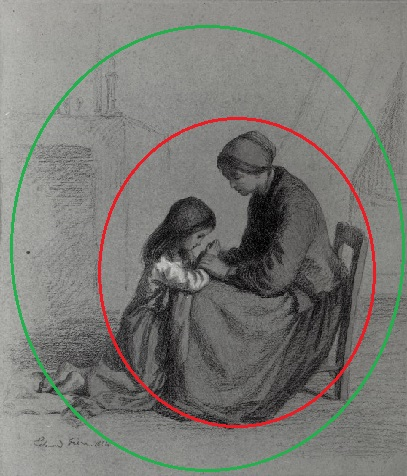
\includegraphics[, scale=0.5]{images/child.jpg}
    \caption{Dibujo donde se muestra el efecto deseado. En rojo se marca el área de interés, en verde la disminución del contraste.\textit{'Child Praying at mothers knee' de Pierre-Édouard Frère }}
    \label{ej_sal}
    \end{figure}
%%%%%%%%%%%%%%%%%%%%%%%%%%%%%%%%






Propuesto por \cite{hata} en su método, se construye una imagen multi-resolución basada en una Pirámide Gaussiana multi contraste y el mapa de saliency.

La pirámide gaussiana se construye disminuyendo iterativamente la resolución de la imagen original y aplicando un filtro gaussiano en cada disminución. La cantidad de imágenes re-escaladas es igual al número de capas de la pirámide.
Una vez realizado este proceso nos apoyamos en el mapa de saliency obtenido para calcular los pixeles que pertenecerán a la imagen multiresolución. Se utiliza la ecuación \ref{mres_1} para calcular la capa a elegir de la pirámide gaussiana

\begin{equation} \label{mres_1}
r = SMX(x,y)(L)
\end{equation}

Donde SMX es el saliency map extendido y L el número de capas de la pirámide. Depués se obtienen los pixeles de la imagen MI interpolando linelmente los valores de los pixeles en las 2 capas adyacentes de la pirámide (Eq. \ref{mi}).

\begin{equation} \label{mi}
MI = (1-a)\cdot PI_{r}(x,y) +  a\cdot PI_{r+1}(x,y)
\end{equation}

Donde a= r-floor(r) y  PI es el valor del pixel (x,y) en la pirámide r y r+1.


\subsection{Generación de trazos a lapiz a partir de extraccion de bordes}
Una primera forma de acercase a generar trazos con apariencia de sketch, de manera automática es utilizar algún método de extracción de bordes. Métodos clásicos como Canny, Sobel son útiles y en ocasiones dan buenos resultados, sin embargo, tienen el problema de ser propensos muy a ruido. Una imagen ruidosa es un enemigo de las imagenes creadas con NPR debido a que 'ensucia' una imagen que busca ser estilizada, además de que en una ilustración hecha a mano alzada dificilmente existe ruido.

Es por ello que se opta por utilizar un operador de gradiente sobre la imagen para tener la información de bordes. Con la ecuación

\begin{equation} \label{grad}
G=((\partial_{x}I)^{2} + (\partial_{y}I)^{2} )^{\frac{1}{2}}
\end{equation}

donde I es la imagen en escala de grises y $\partial_{x}$, $\partial_{y}$ los operadores de gradiente en diección x y y.

La información de borde es importante para obtener la forma general de los trazos. Lo siguiente es procesarla para conseguir una línea que asemeje el trazo de un dibujo a mano alzada.
Los trazos típicos tienen distorsiones, cruces y discontinuidades en las líneas. Un sketch es un dibujo rápido y la consistencia y pulso de sus líneas varía. Típicos trazos en un dibujo de sketch se muestran en la figura \ref{sketch}

%%%%%%%%%%imagen
\begin{figure}[H]
\centering
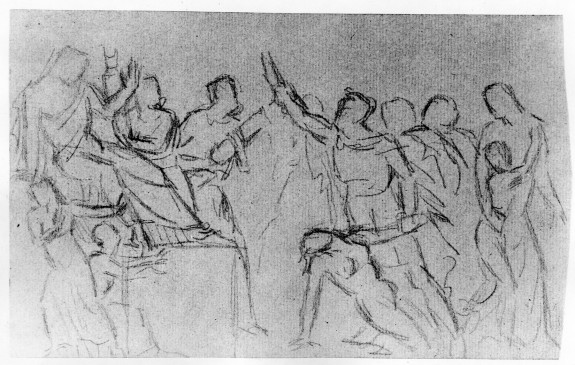
\includegraphics[width=\linewidth, scale=0.1]{images/study_111.jpg}

\caption{Trazos típicos en un Sketch. \textit{'Study after classical scene' De Antoine-Louis Barye}}
    \label{sketch}
    \end{figure}
%%%%%%%%%%%%%%%%%%%%%%%%%%%%%%%%%%%%%%%%%%%%%

Con esta idea en mente se propone un kernel convolucional que extraiga la información de los bordes en 8 direcciones distintas. Para determinar la respuesta se crea el set ${\Lambda_{i}}, i\in {1, ..., 8}$, que contiene un kernel rotado de 0 a 180º en 8 direcciones. La longitud del kernel es variable, pero se recomienda un tamaño de 1/30 de la imagen.


\begin{equation} \label{}
G= \Lambda_{i} * G
\end{equation}

Después de obtener la convolución se forma una Clasificación donde el valor más alto de todas las capas de G es elegido para ese picel y los valores del resto de direcciones son considerados como cero


\begin{equation} \label{}
G_{i}(p)= \left\{ \begin{array}{rcl}
G(p)& \mbox{si}
& argmax(G_{i}(p))=i \\ 0 &  & c.o.c
\end{array}\right.
\end{equation}

La respuesta resultante es convolucionada otra vez en una dirección para crear un efecto de cruce entre líneas. El valor máximo de las ocho direcciones es filtrado y finalmente combinado.En la figura \ref{kernel} se muestra un ejemplo de como se ven estas líneas durante este proceso

%%%%%%%%%%imagen
\begin{figure}[H]
\centering
    \begin{subfigure}{0.45\linewidth}
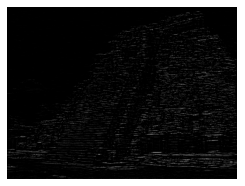
\includegraphics[width=\linewidth, scale=0.05]{images/stroke_0.png} 
    \caption{$\Lambda_{1}$}
\label{fig:1a}
    \end{subfigure}\hfill
    \begin{subfigure}{0.45\linewidth}
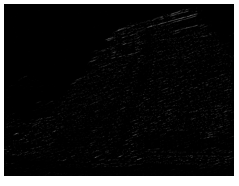
\includegraphics[width=\linewidth, scale=0.1]{images/stroke_1.png}
    \caption{$\Lambda_{2}$}
\label{fig:1a}
    \end{subfigure}

    \begin{subfigure}{0.45\linewidth}
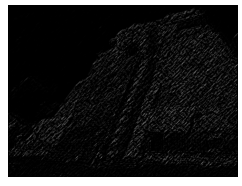
\includegraphics[width=\linewidth,scale=1.2]{images/stroke_2.png}
    \caption{$\Lambda_{3}$}
\label{fig:1a}
    \end{subfigure}\hfill
    \begin{subfigure}{0.45\linewidth}
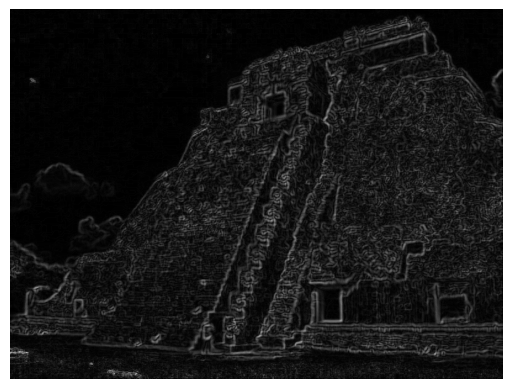
\includegraphics[width=\linewidth,scale=1.2]{images/stroke_3.png}
    \caption{Mapa de trazos combinado}
\label{kernel-d}
    \end{subfigure}
\caption{Kernel convolucional direccional}
    \label{kernel}
    \end{figure}

Como se observa en \ref{kernel-d} la imagen obtenida está invertida por lo que invertir la imagen sería el paso final para obtener un mapa de trazos.

\subsection{Generación de sombreado con un mapa de tonos y textura}

Al hacer un análisis del histograma en dibujos realizados con lápiz sobre papel, se puede notar que los dibujos con esta técnica presentan características propias diferentes a las de una fotografía a escala de grises. Un ejemplo de ello se muestra en la figura\ref{comp-hist}, donde se comparan 2 imágenes con estructura similar.
Esto da la pista de que para buscar una apariencia de sketch es necesario acercarse al tipo de tono común en este tipo de ilustraciones.

%%%%%%%%%%imagen
\begin{figure}
\centering
    \begin{subfigure}{0.45\linewidth}
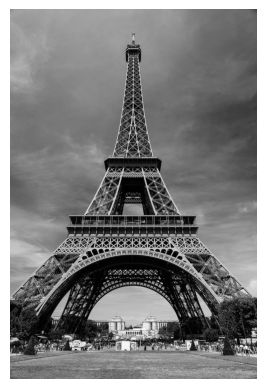
\includegraphics[, scale=0.5]{images/torre_f.png} 
    \caption{Fotografía a escala de grises}
\label{fig:1a}
    \end{subfigure}\hfill
    \begin{subfigure}{0.45\linewidth}
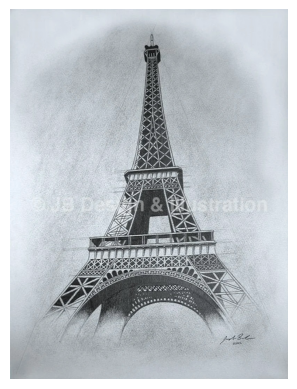
\includegraphics[width=\linewidth, scale=0.1]{images/torre_d.png}
    \caption{Dibujo a lápiz}
\label{fig:1a}
    \end{subfigure}

    \begin{subfigure}{0.45\linewidth}
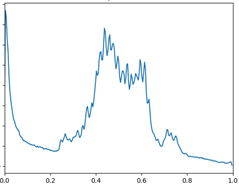
\includegraphics[width=\linewidth,scale=1.2]{images/torre_f_hist.png}
    \caption{Histograma a (a)}
\label{fig:1a}
    \end{subfigure}\hfill
    \begin{subfigure}{0.45\linewidth}
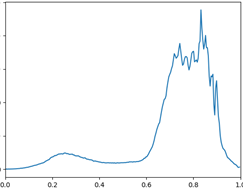
\includegraphics[width=\linewidth,scale=1.2]{images/torre_d_hist.png}
    \caption{Histograma de (b)}
\label{fig:1a}
    \end{subfigure}
\caption{Comparación entre histograma de una fotografía y un dibujo a lápiz. Se eligieron imágenes muy similares para la comparación. Se puede notar que (d) presenta menos variaciones que (a), además de una curva que es común para dibujos a lápiz}
    \label{comp-hist}
    \end{figure}

Siguiendo con la misma idea, en la técnica de dibujo es común aprender a trazar y a diferenciar una escala de tonos posibles de crear con el lápiz (fig \ref{uno})

Lu et al\cite{lu} presentó un modelo para clasificar y aproximarse a este tipo de tonos, clasificándolos como Oscuros, medios y blancos.
En fig. \ref{uno} se puede ver los histogramas comunes para cada tipo de tono


\begin{figure}
\centering
    \begin{subfigure}{0.45\linewidth}
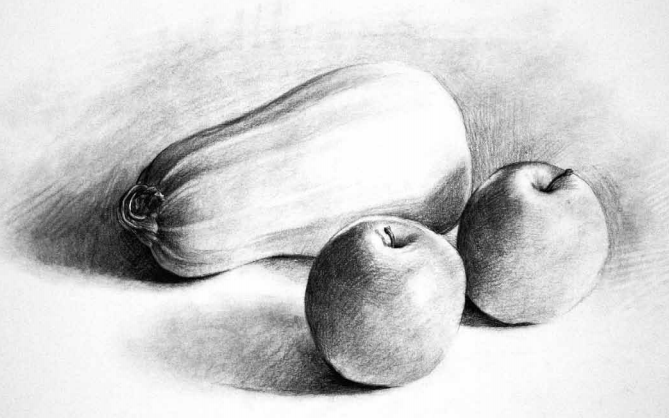
\includegraphics[width=\linewidth, scale=0.05]{images/tone_im.png} 
    \caption{Dibujo a lapiz donde s observan los diferentes tonos que se generan en este tipo de imágenes.}
\label{fig:1a}
    \end{subfigure}\hfill
    \begin{subfigure}{0.45\linewidth}
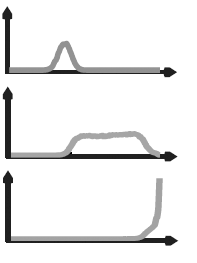
\includegraphics[width=\linewidth, scale=0.1]{images/tone_ex_hist.png}
    \caption{Histogramas de los 3 tipos de todos. En orden: Tonos oscuros, medios y blancos}
\label{dib-hist}
    \end{subfigure}\vfill
    \begin{subfigure}{0.45\linewidth}
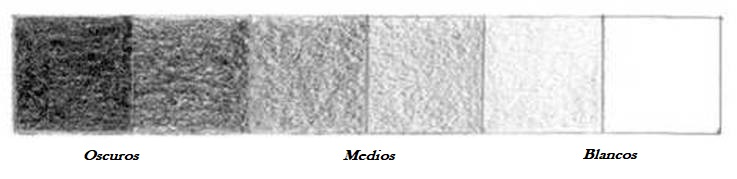
\includegraphics[width=\linewidth, scale=0.1]{images/value.jpg}
    \caption{Escala de tonos generada por un lápiz}
\label{fig:1a}
    \end{subfigure}
\caption{Trazos típicos en un Sketch}
\label{uno}
    \end{figure}

Para modelar esto se propone un modelo paramétrico.


\begin{equation} \label{mod}
p(v)= \frac{1}{N} \sum_{i=1}^{3} w_{i}p_{i}(v)
\end{equation}

donde v es el valor de tono, p(v) la probabilidad de que en un pixel exista el valor v, N es un factor de normalización y w son pesos asociados al númnero de pixeles pertenecientes a cada rgupo de tonos.

El siguiente paso es modelar cada tipo de tono. Retomando la fig. \ref{dib-hist} para los tonos oscuros se propone una distribución gaussiana:

\begin{equation} \label{pa1}
p_{1}(v)= \frac{1}{\sqrt{2\pi\sigma_{d}}} e^{-\frac{(v-\mu_{d})^{2}}{2\sigma_{d}^{2}}    }  
\end{equation}

Para los tonos medios se propone una distribución uniforme

\begin{equation} \label{pa2}
p_{2}(v)= \left\{ \begin{array}{rcl}
\frac{1}{u_{b} - u_{a} }     & \mbox{si}
& u_{a} \leq v \leq u_{b} \\ 0 &  & c.o.c
\end{array}\right.
\end{equation}

Y para los blancos una distribución Laplaciana

\begin{equation} \label{pa}
p_{3}(v)= \left\{ \begin{array}{rcl}
\frac{1}{\sigma_{b}}e^{\frac{1_v}{\sigma_{b}}}     & \mbox{si}
& v \leq 1 \\ 0  &  & c.o.c
\end{array}\right.
\end{equation}



\subsubsection{Estimación de parámetros}
Para ajustar las distribuciones a nuestra información \cite{lu} propone utilizar el método estadístico de estimación de parámetros Maximum Likehood Estimatiton.

En este trabajo se retoman los valores propuestos por \cite{lu} para recrear el modelo paramétrico. Estos parámetros se muestran en la fig. \ref{param}

\begin{figure}[H]
\centering 
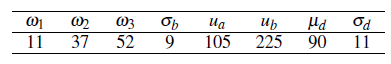
\includegraphics[width=\linewidth, scale=0.05]{images/param.png} 
\caption{Parámetros aprendidos en estimación de \cite{lu}}
    \label{param}
    \end{figure}

\subsubsection{Histogram matching}

Una vez obtenido el modelo adecuado de tonos se hace un emparejamiento de histogramas con la imagen a procesar.

Para ello se utilza el método de Group mapping law, se calcula la función distribuida acumulativa del histograma de la imagen de entrada y del histograma del modelo con parámetros aprendidos, después se mapea de uno a otro.



\subsection{Pencil Rendering}

Finalmente se crea el renderizado de lápiz por medio de una textura H. Se utiliza la siguiente ecuación

\begin{equation} \label{rend}
H(x)^{\beta(x)}  \approx J(x)
\end{equation}

Lo que se expresa es que se busca aproximar el mapa de tonos J trazando $\beta$ veces una imagen de textura H. Expresado en su forma logarítmica se tiene  $\beta(x)lnH(x) \approx lnJ(x)$. Ecuanción que se puede resolver para beta por el método del gradiente conjugado.

Ya calculado el valor $\beta$ el mapa final de textura T se calcula como:


\begin{equation} \label{grad}
T=H^{\beta}
\end{equation}

donde las texturas H propuestas fueron dibujadas a lápiz y se muestran en \ref{textura}


\begin{figure}[H]
\centering
    \begin{subfigure}{0.45\linewidth}
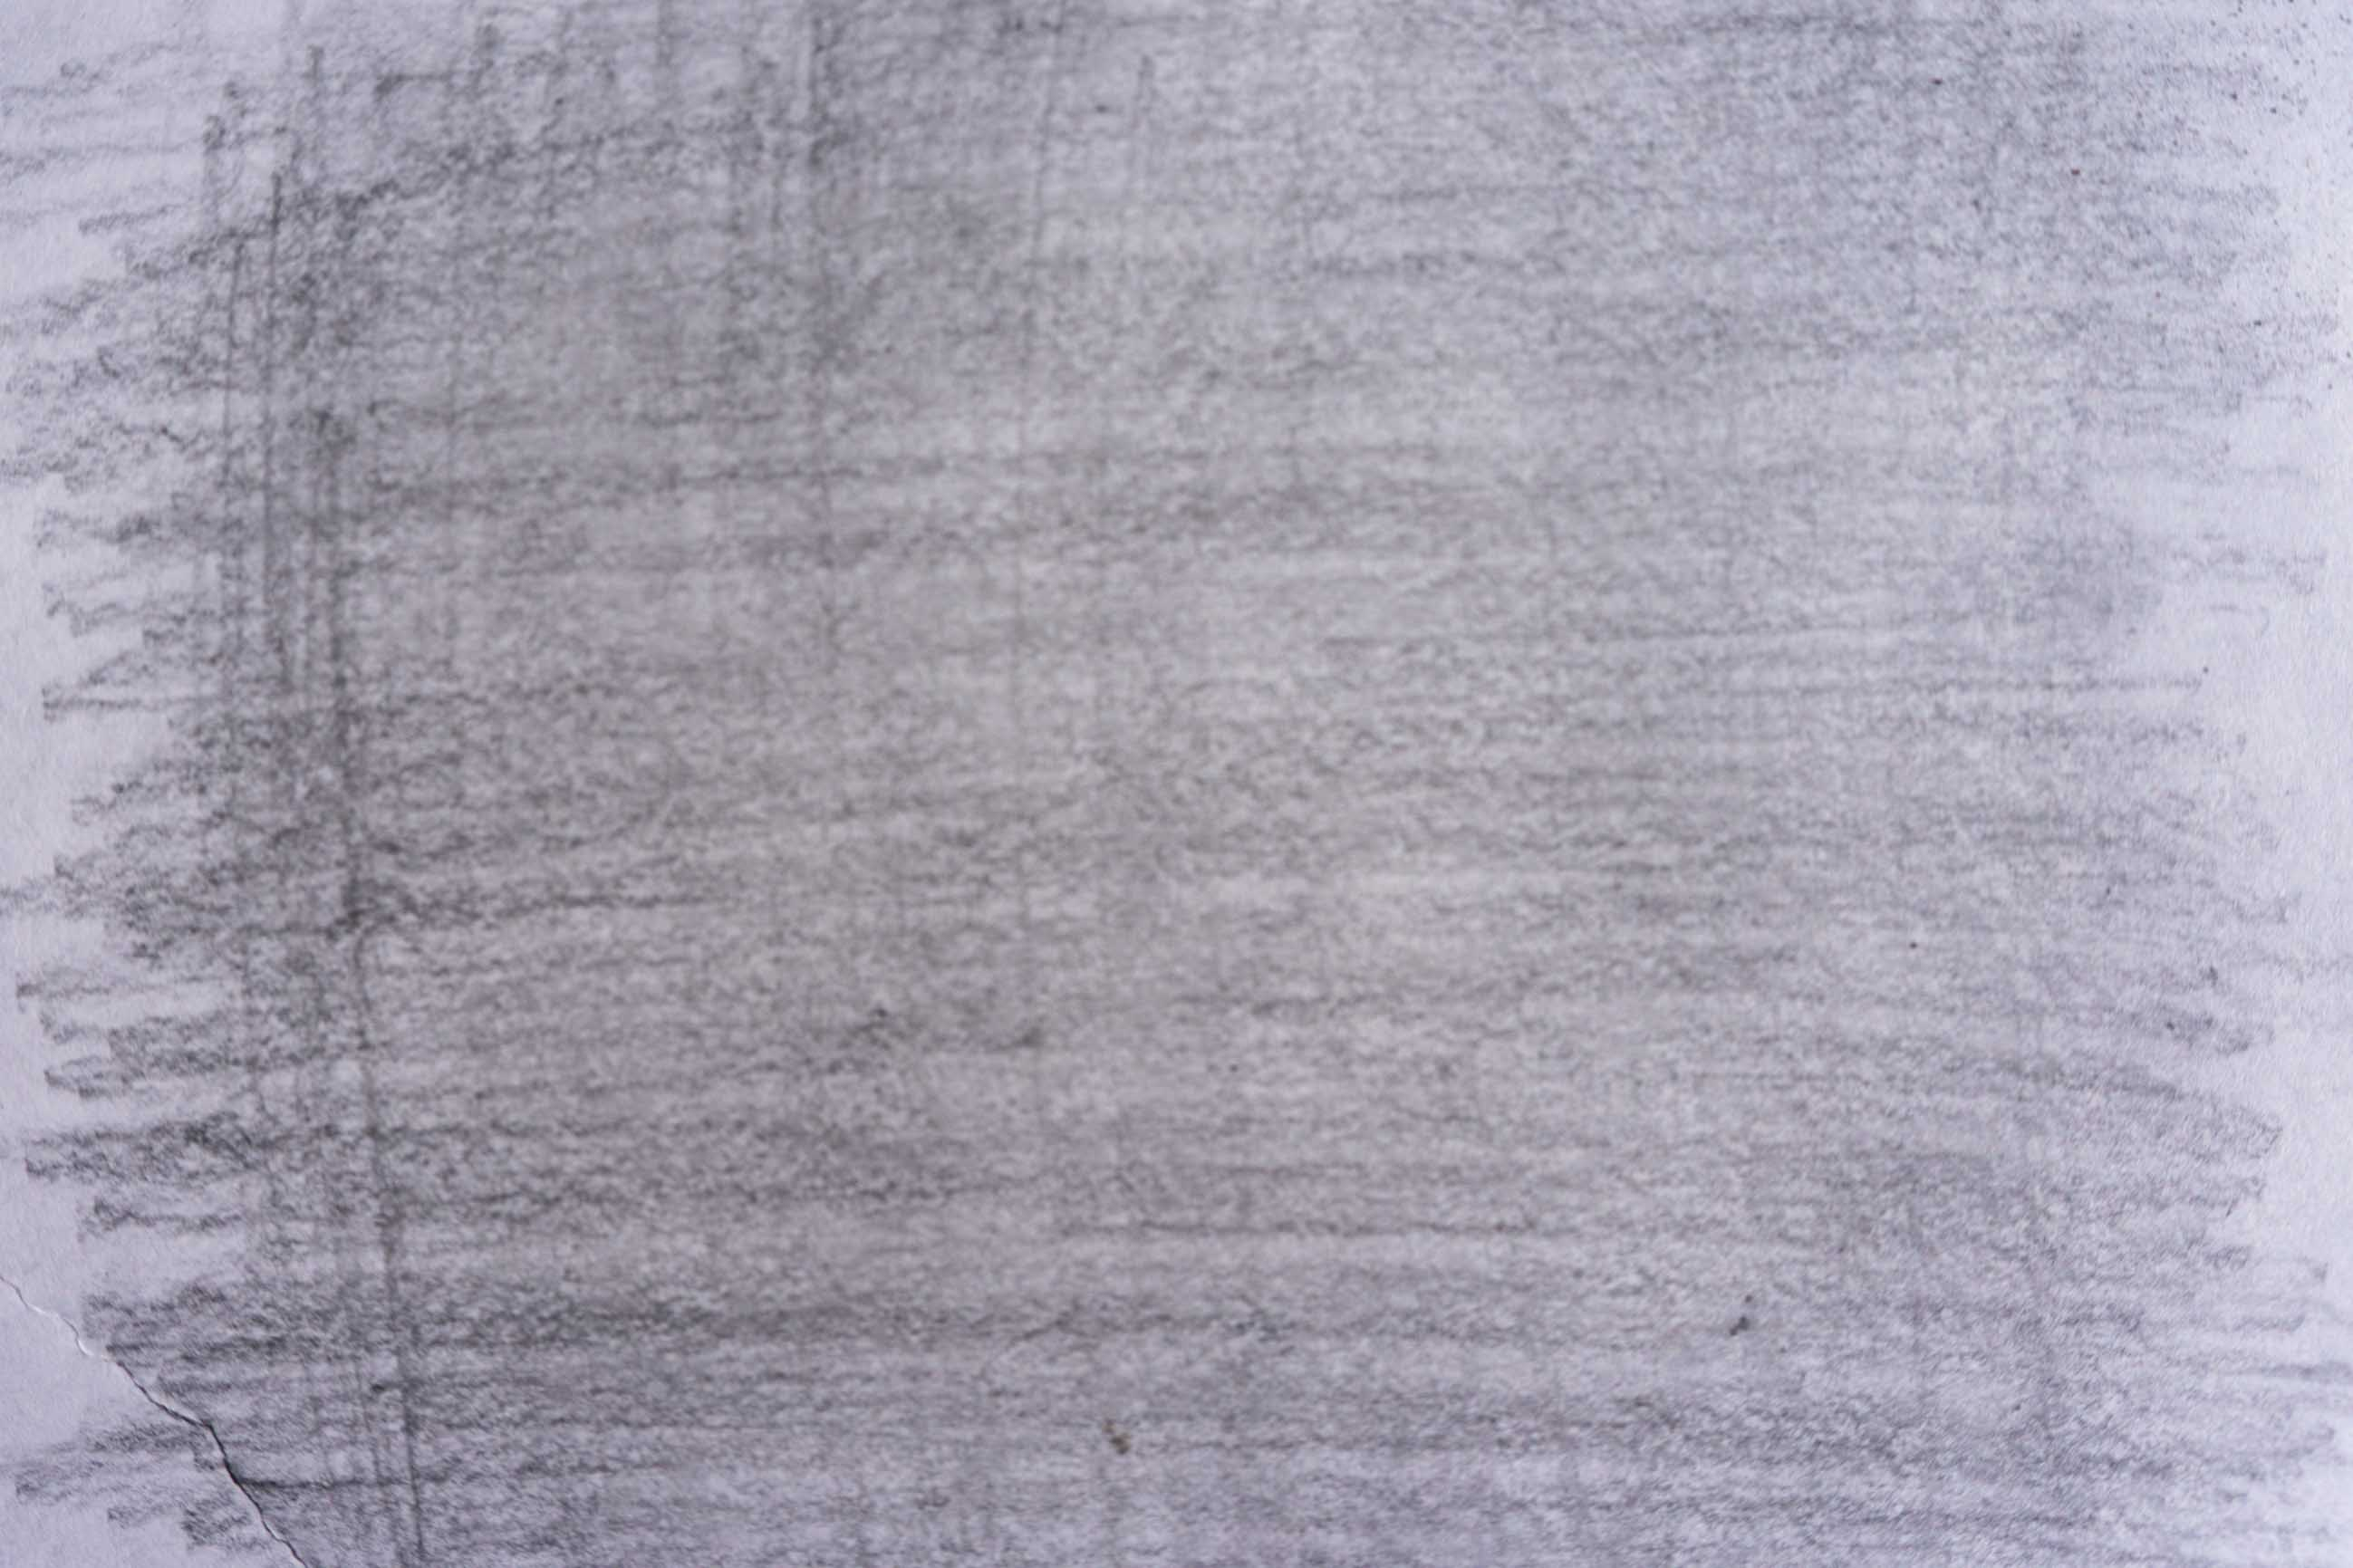
\includegraphics[width=\linewidth, scale=0.05]{images/texture_1.jpg} 
    \caption{Textura de lápiz 1}
\label{fig:1a}
    \end{subfigure}\hfill
    \begin{subfigure}{0.45\linewidth}
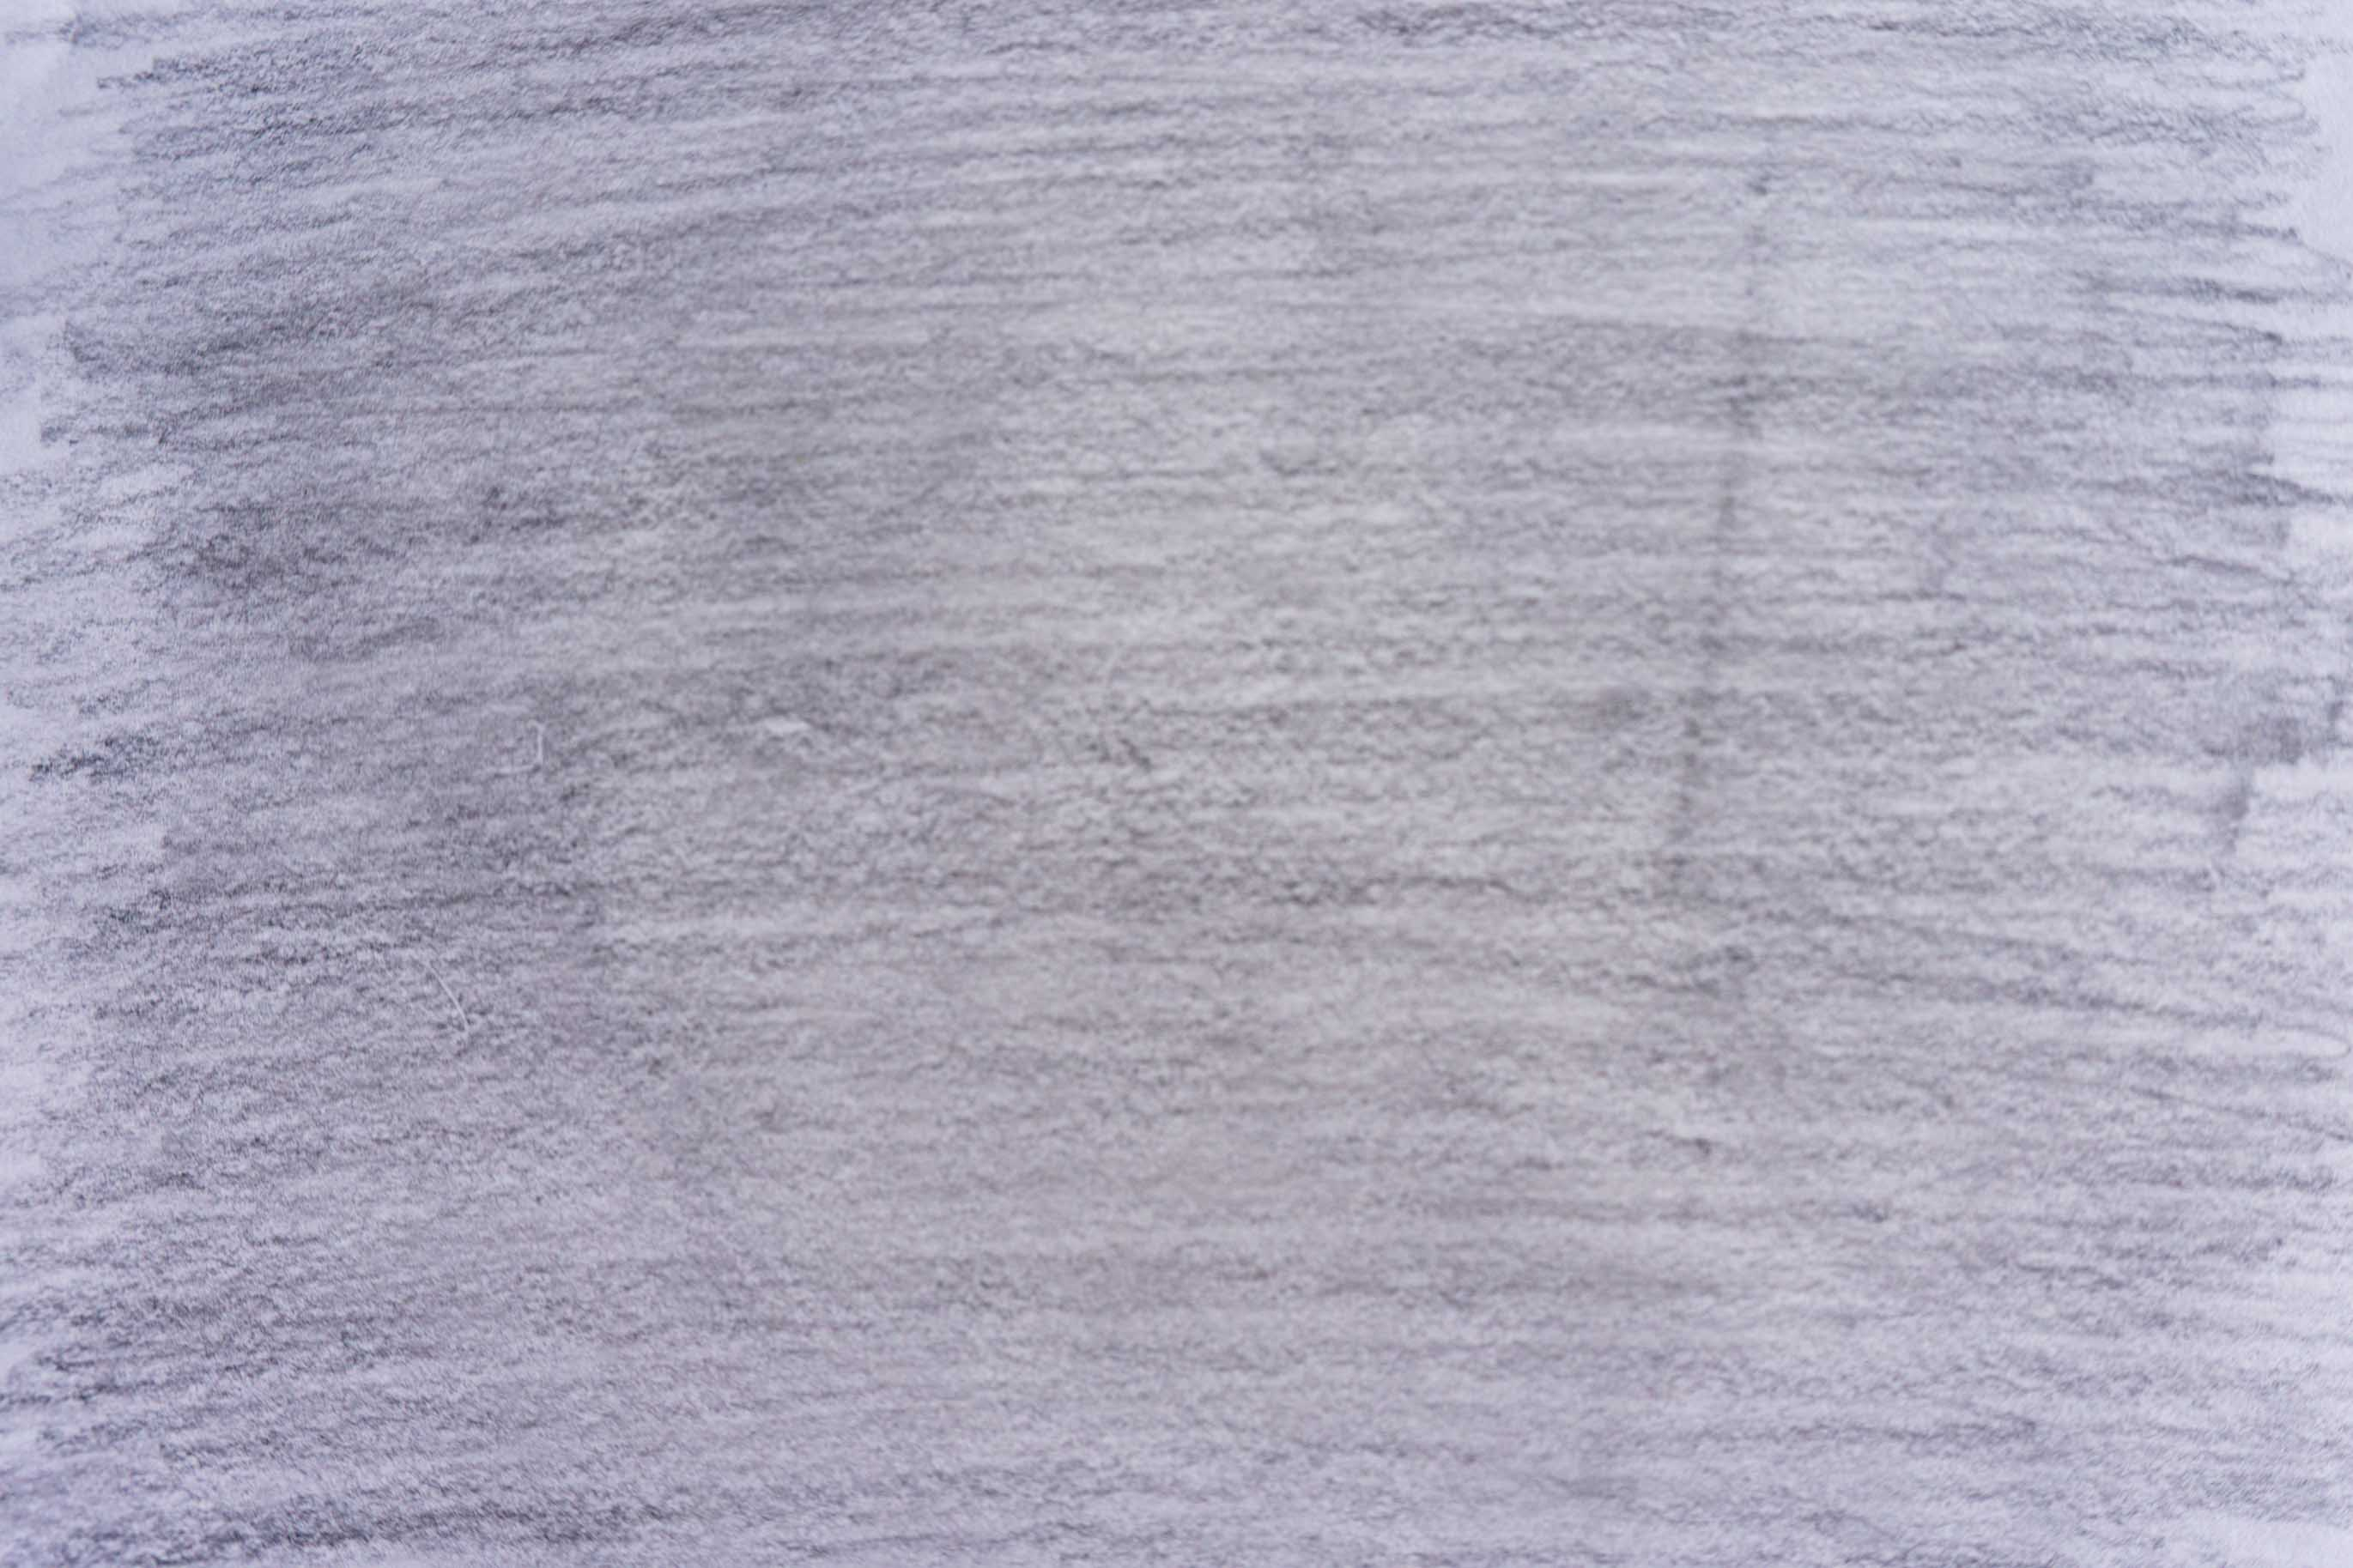
\includegraphics[width=\linewidth, scale=0.1]{images/texture_2.jpg}
    \caption{Textura de lápiz 2}
\label{dib-hist}
    \end{subfigure}
\caption{Texturas utilizadas para el renderizado.}
    \label{textura}
    \end{figure}





\section{RESULTS}

\subsection{Implementación}
Se implemenetó la técnica propuesta en Python con Jupyter notebook. Para calcular el mapa de saliency se utilizó la biblioteca de OpenCV. La pirámide Gaussiana fue implemendata con 3 capas. Los parámetros utilizados para la generación del histograma fueron los propuestos por \cite{lu}. El gradiente conjugado se calculó con matrices dispersas y la biblioteca de Scipy. La galería de imágenes presentadas se tomó de la base de dato presentada por \cite{lu}


\section{Resultados}

El método entregó resultados como la figura 9.
\begin{figure}[H]
\centering
    \begin{subfigure}{0.45\linewidth}
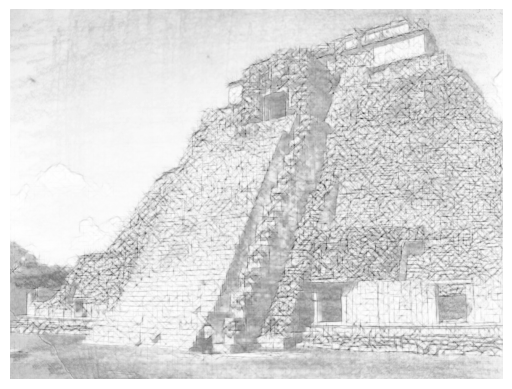
\includegraphics[width=\linewidth, scale=0.05]{images/res_gray.png} 
    \caption{Resultado de texturizado con imagen en escala de grises}
\label{fig:1a}
    \end{subfigure}\hfill
    \begin{subfigure}{0.45\linewidth}
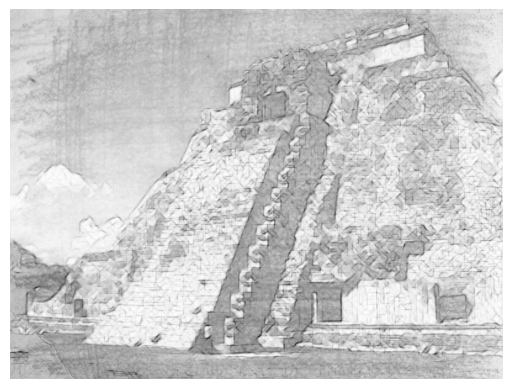
\includegraphics[width=\linewidth, scale=0.1]{images/res_mres.png}
    \caption{Resultado de texturizado con imagen multi-resolución}
\label{dib-hist}
    \end{subfigure}
\caption{Resultados método propuesto}
\label{porfavor}
    \end{figure}
    
Como el cambio en el contraste no fue el esperado se propuso el paso extra de aplicarle a la imagen una máscara binaria creando un mapa de saliency binario. El resultado es el de la figura 10.

\begin{figure}[H]
\centering
    \begin{subfigure}{0.45\linewidth}

\includegraphics[width=\linewidth, scale=0.05]{images/sal_bin.png} 
    \caption{Máscara binaria aplicada al mapa de tonos paara buscar un mayor contraste}
\label{fig:1a}
    \end{subfigure}\hfill
    \begin{subfigure}{0.45\linewidth}
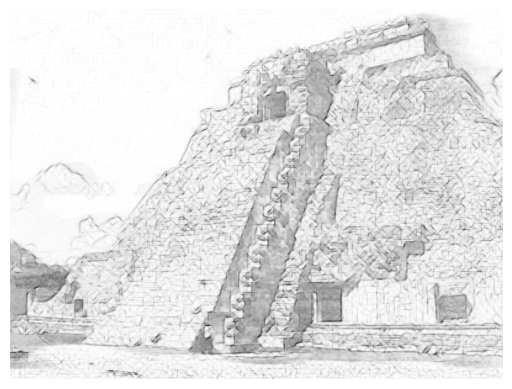
\includegraphics[width=\linewidth, scale=0.1]{images/res_bin.png}
    \caption{Resultado de texturizado con imagen de máscara binaria}
\label{dib-hist}
    \end{subfigure}
\caption{Resultados método propuesto alternativo}
    \label{res1}
    \end{figure}

\subsubsection{Evaluación}
Para una evaluación cuantitativa se compararon nuestros 3 métodos propuestos. Se realizó un cuestionario a 50 personas donde se les pidió que evaluaran la estética de la imagen, su parecido con un skecth a lápiz, y el éxito del método en recrear la imagen original. También, para conocer a la población, se les pidió que indicaran del 1 al 5 su experiencia con artes plásticas y fotografía.

Los resultados se muestran en la tabla \ref{res1}
  
\begin{table}[H]

\begin{tabular}{cccc}

\hline
\textbf{}                 & \multicolumn{3}{c}{\textbf{Evaluación}}                                                                           \\ \hline
\textbf{Método}           & \textbf{Estética} & \multicolumn{1}{l}{\textbf{Parecido Sketch}} & \multicolumn{1}{l}{\textbf{Parecido original}} \\ \hline
\textbf{Escala de grises} & 46\%              & 36.5\%                                       & 41.5\%                                         \\ \hline
\textbf{Multi-contraste}  & 37\%              & 25\%                                         & 50\%                                           \\ \hline
\textbf{Máscara binaria}  & 17\%              & 38.5\%                                       & 8.5\%                                          \\ \hline
\end{tabular}

  \caption{Comparación entre métodos desarrolados. Resultados de encuesta}
  \label{res1}

\end{table}

Por otro lado se compararon resultados del método propuesto con el método de Lu\cite{lu}, el software de Photoshop CC2015 de Adobe y la app para celular Pencil Photo Sketch Editor de Minerva Studio, con mas de 200 mil opiniones positivas. Estos resultados se muestran en \ref{res2}.


\begin{figure}[H]
\centering
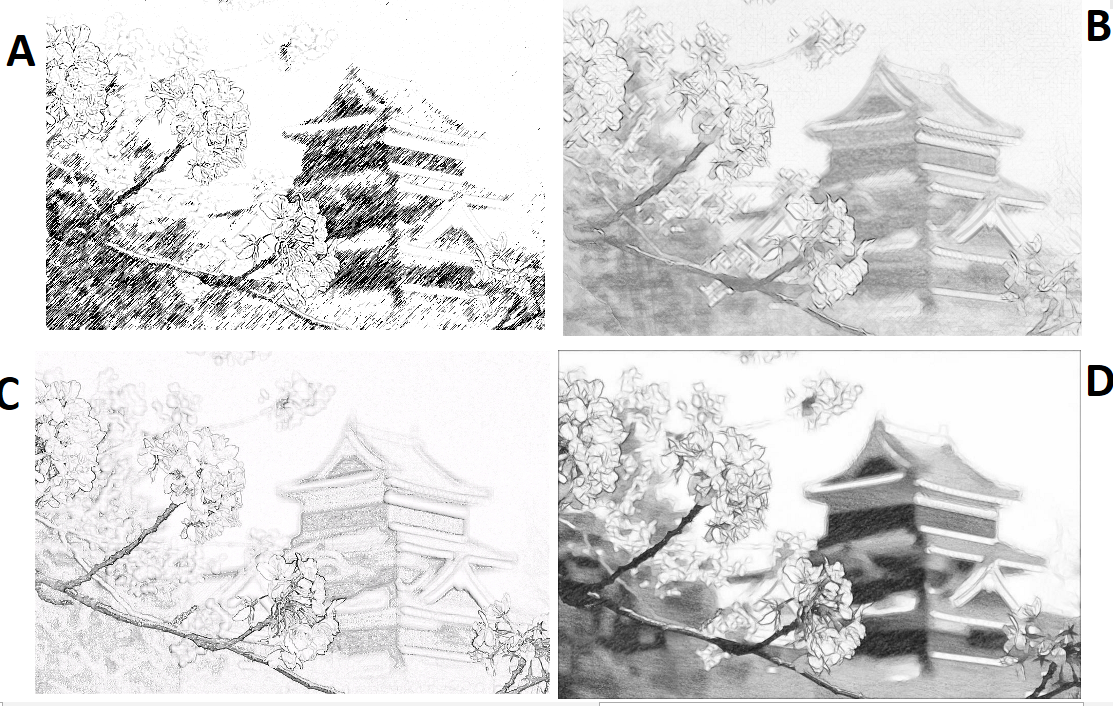
\includegraphics[width=\linewidth, scale=0.05]{images/2--43.png} 
\caption{Comparación entre métodos. A) Photoshop, B) Propuesto, C)App, D)Lu etal\cite{lu}}
    \label{comp}
    \end{figure}


\begin{table}[H]
\centering
\begin{tabular}{ccc}
\hline
\textbf{}                      & \multicolumn{2}{c}{\textbf{Evaluación}}                          \\ \hline
\textbf{Método}                & \textbf{Estética} & \multicolumn{1}{l}{\textbf{Parecido Sketch}} \\ \hline
\textit{\textbf{Lu}}           & 34.4\%            & 22.9\%                                       \\ \hline
\textit{\textbf{Photoshop CC}} & 20.9\%            & 27.1\%                                       \\ \hline
\textit{\textbf{App}}          & 21.8\%            & 26.9\%                                       \\ \hline
\textit{\textbf{Propuesto}}    & 22.9\%            & 23.1\%                                      
\end{tabular}

  \caption{Comparación con otros métodos. Resultados de encuesta}
  \label{res2}
\end{table}



\section{DISCUSIÓN \& CONCLUSIONES}

La evaluación muestra una cierta preferencia por la imagen procesada en escala de grises en cuanto a estética, sin embargo, los otros dos metodos resaltan en parecido a sketch y recreación de la imagen original. Para el caso de la imagen con máscara binaria, es probable que los encuestados relacionarán la imagen con menor detalle y apariencia de estar incompleta con la de un sketch. Esto era justo lo que se buscaba por lo que la aplicación de la máscara cumplió con su cometido.
Por otro lado la imagen multiresolucón mostro un mayor contraste en las líneas lo que causó una asoción con el parecido de la imagen original.

Se debe considerar que hay imagenes en que el mapa de saliency no logra rescatar con exactitud el area de interés buscada. Obtener información de saliency es un reto dificil en el campo de visión que aun se sigue estudiando. Estos resultados dan pie a seguir trabajando con nuevos métodos basados en saliency y en adecuar su funcionamiento a encontrar regiones de interés amplias como las que buscamos.

Finalmente, en la comparación con otros métodos es interesante notar que los encuestados parecen haber relacionado una baja estética con un alto parecido a sketch. Dentro de ello nuestro método se mantuvo como el segundo con mejor estética, detrás de \cite{lu}. 

Cabe destacar que ninguna de las poblaciones tenía experiencia en dibujo o fotografía por lo que queda como tarea a futuro realizar la encuesta en una población más diversa y con mayor experiencia en análisis de imágenes.


\addtolength{\textheight}{-12cm}   % This command serves to balance the column lengths
                                  % on the last page of the document manually. It shortens
                                  % the textheight of the last page by a suitable amount.
                                  % This command does not take effect until the next page
                                  % so it should come on the page before the last. Make
                                  % sure that you do not shorten the textheight too much.

%%%%%%%%%%%%%%%%%%%%%%%%%%%%%%%%%%%%%%%%%%%%%%%%%%%%%%%%%%%%%%%%%%%%%%%%%%%%%%%%



%%%%%%%%%%%%%%%%%%%%%%%%%%%%%%%%%%%%%%%%%%%%%%%%%%%%%%%%%%%%%%%%%%%%%%%%%%%%%%%%



%%%%%%%%%%%%%%%%%%%%%%%%%%%%%%%%%%%%%%%%%%%%%%%%%%%%%%%%%%%%%%%%%%%%%%%%%%%%%%%
%%%%%%%%%%%%%%%%%%%%%%%%%%%%%%%%%%%%%%%%%%%%%%%%%%%%%%%%%%%%%%%%%%%%%%%%%%%%%%%%


\begin{thebibliography}{99}

\bibitem{lu} C. Lu, L. Xu, and J. Jia, “Combining Sketch and Tone for Pencil Drawing Production,”

\bibitem{hata} M. Hata, M. Toyoura, and X. Mao, “Automatic generation of accentuated pencil drawing with saliency map and LIC,” Vis Comput, vol. 28, no. 6–8, pp. 657–668, Jun. 2012, doi: 10.1007/s00371-012-0689-9.

\bibitem{hou} X. Hou and L. Zhang, “Saliency Detection: A Spectral Residual Approach,” in 2007 IEEE Conference on Computer Vision and Pattern Recognition, Minneapolis, MN, USA, Jun. 2007, pp. 1–8. doi: 10.1109/CVPR.2007.383267.

\bibitem{mao} X. Mao, Y. Nagasaka, and A. Imamiya, “Automatic generation of pencil drawing using LIC,” in ACM SIGGRAPH 2002 conference abstracts and applications on   - SIGGRAPH ’02, San Antonio, Texas, 2002, p. 149. doi: 10.1145/1242073.1242162.

\bibitem{dec} A. Santella and D. DeCarlo, “Visual interest and NPR: an evaluation and manifesto,” in Proceedings of the 3rd international symposium on Non-photorealistic animation and rendering  - NPAR ’04, Annecy, France, 2004, p. 71. doi: 10.1145/987657.987669.

\bibitem{dec2} D. DeCarlo and A. Santella, “Stylization and Abstraction of Photographs,” p. 8.

\bibitem{zheng} Y. Zheng, Y. Chen, and M. Sarem, “A Novel Pencil Drawing Algorithm Based on Non-Symmetry and Anti-Packing Pattern Representation Model,” IEEE Access, vol. 7, pp. 184950–184962, 2019, doi: 10.1109/ACCESS.2019.2960877.

\bibitem{li} Y. Li, C. Fang, A. Hertzmann, E. Shechtman, and M.-H. Yang, “Im2Pencil: Controllable Pencil Illustration from Photographs,” arXiv:1903.08682 [cs], Mar. 2019, Accessed: Sep. 12, 2021. [Online]. Available: http://arxiv.org/abs/1903.08682

\end{thebibliography}



\end{document}
